\chapter{New Data Integration Abstractions for Agile Web Application Development}
\label{synapse:ch:synapse}

\section{Abstract}

The growing demand for data-driven features in today's Web applications -- such
as targeting, recommendations, or predictions -- has transformed those
applications into complex conglomerates of services operating on each others'
data and lacking integration into a coherent, manageable architecture. We
present {\em \synapse}, an easy-to-use, strong-semantic system for
large-scale, data-driven Web service integration. \synapse lets independent
services cleanly share data with each other in an isolated and scalable way.
The services run on top of their own databases, whose layouts, and engines can
be completely different, and incorporate read-only views of each others' shared
data. \synapse synchronizes these views in real-time using a new scalable,
consistent replication mechanism that leverages the high-level data models in
popular MVC-based Web applications to replicate data across heterogeneous
databases. We have developed \synapse on top of the popular Web framework
Ruby-on-Rails. It supports data replication among a wide variety of SQL and
NoSQL databases, including MySQL, Oracle, PostgreSQL, MongoDB, Cassandra,
Neo4j, and Elasticsearch. We and others have built over a dozen applications
using \synapse with great ease, some of which are running in production with
over 450,000 users.

\section{Introduction}
\label{synapse:sec:intro}

We live in a data-driven world. Web applications today -- from
the simplest smartphone game to the Web's most complex application -- strive to
acquire and integrate data into new, value-added services. Data -- such as user
actions, social information, or locations -- can improve business revenues by
enabling effective product placement and targeted advertisements. It can enhance
user experience by letting applications predict and seamlessly adapt to present
user needs and preferences. It can enable a host of useful
value-added features, such as recommendations for what to search for, what to
buy, where to eat, or what to view. Agility and ease of integration of new data
types and data-driven services are key requirements in this emerging data-driven
Web world.

Unfortunately, creating and evolving data-driven Web applications is
difficult due to the lack of a coherent data architecture for
Web applications. A typical Web application starts out as some core
application logic backed by a single database (DB) backend.
As data-driven features are added, the application's architecture becomes increasingly complex.
The user base grows to a point where performance indexes drive developers to
denormalize data. As features are removed and added, the DB becomes
bloated, making it increasingly difficult to manage and evolve.
To make matters worse, different data-driven features often require different
data layouts on disk and even different DB engines.
For example, graph-oriented DBs, such as Neo4j and Titan, optimize for
traversal of graph data and are often used to implement recommendation
systems~\cite{db-revolution}; search-oriented DBs, such as
Elasticsearch and Solr, offer great performance for textual searches; and
column-oriented DBs, such as Cassandra and HBase,
are optimized for high write throughput.

Because of the need to effectively manage, evolve, and specialize
DBs to support new data-driven features, Web applications
are increasingly built using a service-oriented architecture that
integrates composable services using a variety and multiplicity of
DBs, including SQL and NoSQL.  Often, the same data, needed by
multiple services, must be replicated across different DB
engines.  These DBs must be maintained in sync, a difficult
problem for which no good, general approach currently exists.  

We present {\em \synapse{}}, an easy-to-use and scalable
cross-DB replication system for simplifying the development and 
evolution of data-driven Web applications.  With \synapse, different
services that operate on the same data but demand
different structures can be developed independently, with their
own DBs. These DBs may differ in schema, indexes, layouts,
and engines, but each can seamlessly integrate subsets of
their data from the others.
\synapse transparently synchronizes these data subsets
in real-time with little to no programmer effort. To use \synapse,
developers generally need only specify declaratively what data to
share with or incorporate from other services in a simple
publish/subscribe model.  The data will then arrive into their DBs
in real-time, at scale, and with delivery semantic guarantees.

\synapse makes this possible by leveraging the same abstractions
that Web programmers already use in widely-used Model-View-Controller
(MVC) Web frameworks, such as Ruby-on-Rails, Python Django, or PHP
Symfony.  Using an MVC paradigm, programmers logically separate an
application into \emph{models}, which describe the data persisted and
manipulated, and \emph{controllers}, which are units of work that
implement business logic and act on the models.
Developers specify what data to share among services within model declarations through \synapse intuitive API.
Models are expressed in
terms of high-level objects (also called \emph{entities}) that are
defined and automatically mapped to a DB via {\em Object/Relational
  Mappers} (ORMs)~\cite{Barcia:2008aa}.  Although different DBs
may need different ORMs, most ORMs expose a common high-level
object API to developers that includes create, read, update, and delete
operations.
\synapse 
leverages this common object API and lets ORMs do the heavy lifting to
provide a cross-DB translation layer among Web services.

\setlength{\tabcolsep}{2pt}
\begin{table}[t]
\centering {\footnotesize
 \vspace{-7pt}
 \begin{tabular}{l l l}
 \toprule {\bf Type} & {\bf Supported Vendors} & {\bf Example use cases} \\
 \midrule
 Relational & PostgreSQL, MySQL, Oracle & Highly structured content\\
 Document & MongoDB,TokuMX, RethinkDB & General purpose\\
 Columnar & Cassandra & Write-intensive workloads\\
 Search & Elasticsearch & Aggregations and analytics\\
 Graph & Neo4j & Social network modeling\\
 \bottomrule
 \end{tabular}}
 \vspace{-9pt}
\caption{{{\bf DB types and vendors supported by \synapse.}}}
\vspace{-4pt}
\label{synapse:tab:supported-orms}
\end{table}
\setlength{\tabcolsep}{4pt}

We have built \synapse on Ruby-on-Rails and use it to demonstrate three
key benefits.  First, \synapse supports the needs of modern Web
applications by enabling them to use many combinations of
\emph{heterogeneous DBs}, both SQL and NoSQL. Table~\ref{synapse:tab:supported-orms}
shows the DBs we support, many of which are very popular.  We show that
adding support for new DBs incurs limited effort, which can be done once and
benefit many applications.  The translation between varied DBs is often
automatic through \synapse and its use of ORMs.  At times, some programmer
involvement may be needed to leverage the full power of specific DBs, but we
find such changes very intuitive and to require few lines of code.

Second, \synapse provides
\emph{programmer simplicity} through a simple programming abstraction
based on a publish/subscribe data sharing model in the context of MVC
Web applications which allows programmers to choose their own data
update semantics to match the needs of Web applications.  Using
\synapse, we have built a dozen or so Web applications involving
widely-used Web components such as the e-commerce platform, Spree, to demonstrate
its ease-of-use, and a startup company has already adopted
\synapse in production and uses it to build and evolve their Web
application ecosystem to support over 450,000 users.  Our
integration and operation experience indicate that \synapse vastly
simplifies the construction and evolution of complex data-driven Web
applications, providing a level of agility that is crucial in this
burgeoning new big-data world.

Finally, \synapse can provide excellent \emph{scalability} with low publisher
overheads and modest update propagation delays; we present some experimental
data showing that \synapse scales well up to 60,000 updates/second for various
workloads.  To achieve these goals, it lets subscribers parallelize their
processing of updates as much as the workload and their semantic needs
permit.

\synapse is the first heterogeneous DB replication system that we are
aware of to satisfy these three goals.  For instance, most traditional
data-warehousing systems are not suitable for real-time integration
\cite{Chan:1999:DSM:319757.319787,10.1109/TKDE.2005.16,Yang:1997:AMV:645923.673657}.
Change capture systems often rely on specific
features provided by SQL DBs (e.g., triggers, transaction logs) that can
limit their applicability to today's broad range of DBs~\cite{databus}.

We release our system open source at \url{https://github.com/promiscuous-io/promiscuous}.
(The system's name was initially Promiscuous, but we have decided to change that
to Synapse. The change is still pending in the repo.)
\section{Background}
\label{synapse:s:motivation}

MVC is widely-used and supported by many Web
frameworks, including Struts (Java), Django (Python), Rails (Ruby),
Symfony (PHP), Enterprise Java Beans (Java), and ASP.NET MVC (.NET).
For example, GitHub, Twitter, and YellowPages are built with Rails,
DailyMotion and Yahoo! Answers are built with Symfony, and Pinterest
and Instragram are built with Django.
In the MVC pattern, applications define data models that describe the 
data used (in terms of entities and attributes), which are then typically
persisted to DBs.  Because the data is persisted to a DB, the 
model is expressed in terms of constructs that can be manipulated by
the DBs.  Since MVC applications interact with DBs via ORMs, ORMs
provide the model definition constructs~\cite{Barcia:2008aa}.

ORMs abstract many DB-related
details and let programmers code in terms of high-level objects, which
generally correspond one-to-one to individual rows, or documents
in the underlying DB.  While
ORMs were initially developed for relational DBs, the concept has lately
been applied to many other types of NoSQL DBs.  

While different ORMs may offer different APIs, at a minimum they must
provide a way to {\em create}, {\em update}, and {\em delete} the objects into
the DB.  For example, an application would typically instantiate an
object, set its attributes in memory, and then invoke the ORM's save
function.  Many ORMs and MVC frameworks also support a notion of 
{\em active models}~\cite{Fowler:2002:PEA:579257}, which allow
developers to specify {\em callbacks} that are invoked before or after
any ORM-based update operation.  

MVC applications define controllers to implement business logic and
act on the data.  Controllers define basic units of work in which data
is read, manipulated, and then written back to DBs.  Applications are
otherwise stateless outside of controllers.  Since Web applications
are typically designed to respond to and interact with users,
controllers typically operate within the context of a 
{\em user session}, which means their logic is applied on a per user
basis. 

\setlength{\tabcolsep}{3pt}
\begin{table}[t]
 \centering {\footnotesize
 \begin{tabular}{l l}
\toprule {\bf Abstraction}               & {\bf Description}                              \\ \midrule
Publisher                                & Service publishing attributes of a model.      \\
Subscriber                               & Service subscribing to attributes of a model.  \\
Decorator                                & Service subscribing and publishing a model.    \\
Ephemeral                                & DB-less publisher.                       \\
Observer                                 & DB-less subscriber.                      \\
Virtual attribute                        & Deterministic functions (can be published).    \\
\bottomrule
 \toprule {\bf API}                       & {\bf Description}                              \\ \midrule
 {\code {\footnotesize publish}},         & Annotations to denote which attributes to      \\
 {\code {\footnotesize subscribe}}        & publish or subscribe.                          \\ \midrule
 {\code {\footnotesize before\_create}},  & Re-purposed active model callbacks for         \\
 {\code {\footnotesize before\_update}},  & subscriber update notification. Similar        \\
 {\code {\footnotesize before\_destroy}}  & callbacks for after\_create/update/destroy.    \\ \midrule
 {\code {\footnotesize with\_read\_dep,}} & Specify explicit dependencies for updates.     \\
 {\code {\footnotesize with\_write\_dep}} &                                                \\ \midrule
 {\code {\footnotesize pub\_delivery\_mode}}   & Config. parameter for
selecting delivery \\
 {\code {\footnotesize sub\_delivery\_mode}}    & semantic. \\ \midrule
 {\code {\footnotesize bootstrap?}}       & Predicate method denoting bootstrap mode.         \\
 \bottomrule
 \end{tabular}
 }
 \vspace{-7pt}
 \caption{{\small {\bf \synapse Abstractions and API.}}}
 \vspace{-2pt}
 \label{synapse:tab:api}
\end{table}

\setlength{\tabcolsep}{4pt}
\section{\synapse API}
\label{synapse:sec:programming-model}

\synapse extends the MVC programming pattern to create an
easy-to-use platform for integrating Web services that use
heterogeneous DBs.  
Because MVC frameworks and ORMs provide common abstractions that are
often used in practice for Web development, \synapse
leverages them to provide a transparent and mostly automatic data
propagation layer.

Using the \synapse API shown in Table~\ref{synapse:tab:api}, developers make
simple modifications to their existing model definitions to share their data
across services. At a high
level, an application that uses \synapse consists of one or more publishers,
and one or more subscribers. Publishers are services that make attributes of
their data models available to subscribers, which maintain their own local,
read-only copies of these attributes. \synapse transparently
synchronizes changes to published models (creations, updates, or deletions of
model instances) from the publisher to the subscriber.  It serializes
updated objects on the publisher, transmits them to the subscriber, deserializes
them there, and saves them through the ORM.

If the subscriber application implements active model callbacks,
\synapse also notifies it of the new updates.  Furthermore, a service can
subscribe to a model, \emph{decorate} that model by adding new
attributes to it, and publish these attributes. Such cascading
of subscribers into publishers can be used to create complex
ecosystems of Web services that subscribe from each other, enhance it
with new attributes, and publish it further.  We find this
programming model very easy to use and useful to support powerful new use
cases as shown in \S\ref{synapse:sec:apps}.
We discuss the \synapse API using Ruby-on-Rails, but similar APIs can be
built for other frameworks.

\subsection{\synapse Abstractions}
\label{synapse:sec:api}

\begingroup
\setlength{\columnsep}{6pt}

\heading{Publishers.}
To publish a model, the developer annotates individual entities or attributes
to specify that they should be shared. The code at the top of
\F\ref{synapse:fig:pub-sub} shows how to publish
\begin{wrapfigure}{r}{0.18\textwidth}
\vspace{-0.2cm}
\begin{minipage}{.18\textwidth}
\begin{lstlisting}[xleftmargin=2pt,framexleftmargin=2pt]
# Publisher side (Pub1).
class User
 `\specialKeyword{publish}` do
  field :name
 end
end
\end{lstlisting}\vspace{-12pt}
\begin{lstlisting}[xleftmargin=2pt,framexleftmargin=2pt]
# Subscriber side (Sub1).
class User
 `\specialKeyword{subscribe}` :from => :Pub1 do
  field :name
 end
end
\end{lstlisting}
\end{minipage}
\vspace{-0.5cm}
\caption{{\footnotesize {\bf Publisher (top), subscriber (bottom).}}}
\vspace{-5pt}
\label{synapse:fig:pub-sub}
\end{wrapfigure}
in Ruby using the {\code publish} keyword, with Synapse-specific code
underlined.  Each published model has a globally unique URI, given by {\code
app\_name/model\_name}.  \synapse generates a publisher file for each
publisher listing the various objects and fields being published and is made
available to developers who want to create subscribers for the published data.
A factory file is also made available for each publisher that provides sample
data for writing integration tests (\S\ref{synapse:sec:testing}).  Other API calls that
can be used by publishers are {\code {\small with\_read\_dep}}, {\code {\small
with\_write\_dep}}, and {\code {\small delivery\_mode}}, all discussed in
\S\ref{synapse:sec:semantics}.

\heading{Subscribers.}
To subscribe to a published model, the developer simply marks the attributes of
interest accordingly.  In \F\ref{synapse:fig:pub-sub}, the code at the bottom
shows how to subscribe in Ruby to the publisher at the top.  Since
model name is the same in the subscriber as the publisher, it does not
need to be explicitly identified in conjunction with the 
{\code subscribe} keyword. 
A subscriber application can subscribe to some or all of a publisher's
models, and can subscribe to models from multiple publishers. While
there may be many subscribers for a given model, there can only be one
publisher (the {\em owner} of that model). The owner is the only
service who can create or delete new instances of the model (a.k.a.,
{\em objects}). Moreover, subscribers cannot update attributes that they
import from other services, although they can update their own
decoration attributes on these models. We enforce this {\em read-only}
subscription model to avoid difficult issues related to concurrent update
conflicts from distinct services.
That said, \synapse handles concurrent updates made from different
\begin{wrapfigure}{r}{0.2\textwidth}
\vspace{-0.2cm}
\begin{minipage}{.2\textwidth}
\begin{lstlisting}[xleftmargin=2pt,framexleftmargin=2pt]
# Notification Subscriber
class User
 `\specialKeyword{subscribe}` from => :PubApp do
  field :name
  field :email
 end
 after_create do
  unless `\specialKeyword{Synapse.bootstrap?}`
   self.send_welcome_email
  end
 end
end
\end{lstlisting}
\end{minipage}
\vspace{-0.5cm}
\caption{{\footnotesize {\bf Callback.}}}
\label{synapse:fig:welcome-email}
\vspace{-5pt}
\end{wrapfigure}
\noindent
servers from the same service.

Subscribers often need to perform some
application-specific processing of updates before applying them to their
DBs. For example, a subscriber may need to compute some new fields,
denormalize some data, or send a notification.  \synapse supports this by
piggybacking upon active model callbacks often supported by MVC frameworks,
including {\code \small before/after\_create}, {\code \small before/after\_update}, or
{\code \small  before/after\_destroy}.
The code on the right shows an after callback example where the subscriber
sends a welcome email for each newly created User.
These callbacks are particularly useful to adapt schemas
between publishers and subscribers, a topic that we discuss in
\S\ref{synapse:sec:examples}.  Other API calls that can be used by subscribers are
{\code {\small bootstrap?}} and {\code {\small delivery\_mode}}, all
discussed in \S\ref{synapse:sec:semantics}.  

\heading{Decorators.}
Decorators are services that subscribe to a
\begin{wrapfigure}{r}{0.2\textwidth}
\vspace{-0.2cm}
\begin{minipage}{.2\textwidth}
\begin{lstlisting}[xleftmargin=2pt,framexleftmargin=2pt]
# Decorator side (Dec2).
class User
 `\specialKeyword{subscribe}` from => :Pub1 do
  field :name
 end
 `\specialKeyword{publish}` do
  field :interests
 end
end
\end{lstlisting}
\end{minipage}\vspace{-9pt}\\
\noindent
\begin{minipage}{.2\textwidth}
\begin{lstlisting}[xleftmargin=2pt,framexleftmargin=2pt]
# Subscriber side (Sub2).
class User
 `\specialKeyword{subscribe}` :from => :Pub1 do
  field :name
 end
 `\specialKeyword{subscribe}` :from => :Dec2 do
  field :interests
 end
end
\end{lstlisting}
\end{minipage}
\vspace{-0.5cm}
\caption{{\footnotesize {\bf Decorator.}}}
\label{synapse:fig:deco}
\vspace{-10pt}
\end{wrapfigure}
\noindent
model and publish new attributes for it.  Conceptually, decorators mix the
publisher and subscriber abstractions.  In  reality, there are subtle
limitations that apply to decorators, prompting us to introduce this new
abstraction that makes the
restrictions explicit.  First, decorators cannot create or delete instances
of a model, because they are not its originators.  Second,
decorators cannot update those attributes of the model that they subscribe
to.  Third, decorators cannot publish attributes that they subscribe to.
Our Decorator abstraction encapsulates and enforces these restrictions.
As an example, the code at the top of \F\ref{synapse:fig:deco} shows a decorator
service, which decorates the User model of an application with the user's
interests.  The data used to compute those interests comes from other sources,
such as social activity, but is omitted here. Other services can then subscribe
to any subset of the model's attributes or decorations by specifying the
originators of those attributes, as shown in the code at the bottom of \F\ref{synapse:fig:deco}.
Using decorators, one can construct complex ecosystems of services
that enhance the data in various ways, as showcased by the examples in
\S\ref{synapse:sec:apps}.

\heading{Ephemerals and Observers.} \synapse aims to support as many use cases
for data-driven integration as possible.  Often times we find it useful to
support integration of not only persisted models but also unpersisted models.
For example, one could define a mailer application that observes user
registrations and sends a welcome message, but does not need to store the data.
Similarly, often times although user-facing services receive user actions
(such as clicks, searches, mouse hovering, etc.), it is backend analytics
services that truly use that information.  Having the front-end application just
pass on (publish) the data onto persisting subscribers is useful in such cases.
\synapse hence lets programmers mix persisted models with {\em ephemerals}
(unpersisted published models)
and/or {\em observers} (unpersisted subscribed models).  Aside from
supporting application-driven needs, unpersisted models are often used to
adapt mismatching data models across heterogeneous DBs, as shown in
\S\ref{synapse:sec:examples}.

\heading{Virtual Attributes.} To perform data translation between ORMs,
\synapse simply calls field getter methods on the publisher side, and then
calls the corresponding field setters on the subscriber side. \synapse
additionally lets programmers introduce getters and setters for attributes
that are not in the DB schema.  We call these programmer-provided attributes
{\em virtual attributes}. Virtual attributes are valuable for schema mappings,
as shown in \S\ref{synapse:sec:examples}.

\endgroup

\subsection{\synapse Delivery Semantics}
\label{synapse:sec:semantics}
Update delivery semantics are an
important part of \synapse's programming model. Different applications
require different levels of semantics.  Some can handle overwritten histories,
others may prefer to see every single update.  Similarly, while some
applications can handle updates in any order, others may expect them in an
order that respects application logic. In support of applications with
different needs, and inspired by well-established prior
art~\cite{Lamport:1978:TCO:359545.359563}, \synapse allows
publishers and subscribers to use the {\code delivery\_mode} keyword
to select among three delivery semantics: {\em global},
{\em causal}, and {\em weak}.  

Global order delivery mode means that all object updates will be
sequentially ordered by the publisher and delivered in that order to
subscribers.  This provides the strongest semantics, but
in practice limits horizontal scaling and is rarely if ever used in
production systems.  

Causal order delivery mode guarantees that all writes performed within
a controller are serialized, and that any object read before a write
becomes a happens-before dependency for that write and that those
dependencies are enforced during delivery.  A publisher can also
declare explicit dependencies using the {\code with\_read\_dep} and
{\code with\_write\_dep} constructs in Table~\ref{synapse:tab:api}.
Furthermore, controllers within the same user session are serialized,
so that all writes performed within the same user session are
serialized.  This guarantee fits the users' expectations, and this
model has been shown to provide causal
consistency~\cite{BSW2004,bolton}.
This mode provides sufficient semantics for many Web applications without the
performance limitations of global order delivery mode, as shown by prior
work~\cite{mahajan11cacTR,cops,eiger} and our evaluation in
\S\ref{synapse:sec:evaluation:delivery}.

Weak order delivery mode always updates objects to their latest
version, but may miss or ignore intermediate updates if they are
delivered out of order.  This ordering may introduce overwritten
histories.  This mode is suitable for applications that have low
semantic requirements.  This mode provides good scaling properties,
but its most important benefit is high availability due to its
tolerance of message loss.  For example, causal order delivery mode
requires delivery of every single update for all objects, so loss
of an update would result in failure.  In production, unfortunately,
situations occur where messages do get lost despite the use of
reliable components (see \S\ref{synapse:sec:eval:ease-of-use}).  Weak
order delivery mode can ignore causal dependencies and only update
to the latest version.

Publishers select the modes that deliver the strongest semantics that
they wish to support for their subscribers, subject to the performance
overheads they can afford.  Subscribers can only select delivery
semantics that are at most as strong as the publishers support.
Subscribers can select for different delivery modes for data coming
from different publishers.  In the most common and practical setting,
a publisher would select to support causal delivery, while the
subscriber may configure either causal or weak delivery. For example,
given a causal mode publisher, a mailer subscriber that sends emails
on the state transitions of a shopping cart would not tolerate
overwritten histories without additional code, although it is
generally tolerable for the mailer service to be unavailable for short
periods of time. The causal semantic would be well fit for
such a subscriber.  In contrast, a real-time analytics service that
aggregates million of rows at once may not care about orders, while
being unavailable, even for short period of time, may damage the
business.  The weak semantic would be sufficient for this subscriber.

There is but one constraint with the choice of delivery mode in
\synapse.  During the bootstrapping period, which occurs when a
subscriber must catch up after a period of unavailability, \synapse
forces the weak semantic (i.e., the subscriber may witness overwritten
histories and out-of-order deliveries).  We signal such periods
clearly to programmers in our API using the {\code bootstrap?}
predicate.  \S\ref{synapse:sec:arch:bootstrapping} describes this situation and
explains how subscribers demanding higher semantics can deal with it. 
\subsection{\synapse Programming by Example}
\label{synapse:sec:examples}

\synapse addresses many of the challenges of heterogeneous-DB applications automatically through its use of ORMs, often being entirely plug-and-play.
In other cases, the programmer may need to perform explicit translations on the subscriber to align the data models.
Our experience suggests that \synapse's abstractions facilitate these translations, and we illustrate our experience using examples showcasing \synapse's usability with each major class of DB: SQL, document, analytic, and graph.

\begin{figure}[t]
\begin{tabular}{c}
\begin{minipage}{.22\textwidth}
\begin{lstlisting}[xleftmargin=1pt,framexleftmargin=1pt]
# Publisher 1 (Pub1).
# Runs on MongoDB.
class User
 include Mongoid::Document
 `\specialKeyword{publish}` do
  field :name
 end
end
\end{lstlisting}
\end{minipage}\vspace{-8pt}\\
\begin{minipage}{.22\textwidth}
\begin{lstlisting}[xleftmargin=1pt,framexleftmargin=1pt]
# Subscriber 1a (Sub1a).
# Runs on any SQL DB.
class User<ActiveRecord::Base
 `\specialKeyword{subscribe}` :from => :Pub1 do
  field :name
 end
end
\end{lstlisting}
\end{minipage}
\end{tabular}\hfill
\begin{tabular}{c}
\begin{minipage}{0.22\textwidth}
\begin{lstlisting}[xleftmargin=1pt,framexleftmargin=1pt]
# Subscriber 1b (Sub1b).
# Runs on Elasticsearch.
class User < Stretcher::Model
 `\specialKeyword{subscribe}` :from => :Pub1 do
  property :name,:analyzer=>:simple
 end
end
\end{lstlisting}
\end{minipage}\vspace{-8pt}\\
\begin{minipage}{0.22\textwidth}
\begin{lstlisting}[xleftmargin=1pt,framexleftmargin=1pt]
# Subscriber 1c (Sub1c).
# Runs on MongoDB.
class User
 include Mongoid::Document
 `\specialKeyword{subscribe}` :from => :Pub1 do
  field :name
 end
end
\end{lstlisting}
\end{minipage}
\end{tabular}
\vspace{-16pt}
\caption{{\bf Example 1: Basic Integration.}
Shows publishing/subscribing examples with actual ORMs.
\synapse code is trivial.  This is the common case in practice.
}
\label{synapse:fig:mongo-to-star}
\end{figure}

\heading{Example 1: Basic Integrations.}  Our experience suggests that most
integrations with \synapse are entirely automatic and require only simple
annotations of what should be published or subscribed, similar to the ones shown
in \F\ref{synapse:fig:pub-sub}.  To showcase, \F\ref{synapse:fig:mongo-to-star} shows the
integration of a MongoDB publisher (Pub1) with three
subscribers: SQL (Sub1a), Elasticsearch (Sub1b), and
MongoDB (Sub1c). The programmers write their models using
the specific syntax that the underlying ORM
provides.  Barring the {\code {\footnotesize publish/subscribe}} keywords, the
models are exactly how each programmer would model them if they were not using
\synapse (i.e., the data were local to their service).  In our experience
building and deploying \synapse, this is by far the most
frequent case of integration.

That said, there are at times more complex situations, where programmers must
intervene to address mismatches between schemas, supported data types, or
optimal layouts.  We find that even in these cases, \synapse provides just the
right abstractions to help the programmer address them easily and elegantly.
We describe next complex examples, which illustrate \synapse's flexibility
and great added value.  We stress that not all integrations between a given DB
pair will face such difficulties, and vice versa, the same difficulty might be
faced between other pairs than those we illustrate.

\begin{figure}
\begin{tabular}{c}
\begin{minipage}{.23\textwidth}
\begin{lstlisting}[xleftmargin=3pt]
# Publisher 2 (Pub2).
# Runs on any SQL DB.
class User<ActiveRecord::Base
 `\specialKeyword{publish}` do
  field :name
  field :likes
 end
 has_many :friendships
end
class Friendship<ActiveRecord::Base
 `\specialKeyword{publish}` do
  belongs_to :user1, :class => User
  belongs_to :user2, :class => User
 end
end
\end{lstlisting}
\end{minipage}\\
\begin{minipage}{.21\textwidth}
\vspace{0.2cm}
\caption{{\bf Example 2: SQL/Neo4j.}
Pub2 (SQL) stores friendships in their own table; Sub2 (Neo4j) stores
them as edges between Users. }
\vspace{-0.2cm}
\label{synapse:fig:sql-to-neo4j}
\end{minipage}
\end{tabular}\hfill
\begin{tabular}{c}
\begin{minipage}{.21\textwidth}
\begin{lstlisting}
# Subscriber 2 (Sub2).
# Runs on Neo4j.
class User  # persisted model
  include Neo4j::ActiveNode
  `\specialKeyword{subscribe}` :from => :Pub2 do
   property :name
   property :likes
  end
  has_many :both, :friends,
   :class => User
end
class Friendship  # not persisted
 include `\specialKeyword{Synapse::Observer}`
 `\specialKeyword{subscribe}` :from => :Pub2 do
  belongs_to :user1, :class => User
  belongs_to :user2, :class => User
 end
 after_create do
  user1.friends << user2
 end
 after_destroy do
  user1.friends.delete(user2)
 end
end
\end{lstlisting}
\end{minipage}
\end{tabular}
\end{figure}

\heading{Example 2: Mapping Data Models with Observers.}
Different DBs model data in different ways so as to optimize different modes of
accessing it. This example shows how to map the data models between a SQL and
Neo4j DB to best leverage the DBs' functions.  Neo4j, a graph-oriented DB, is
optimized for graph-structured data and queries. It stores relationships between
data items -- such as users in a social network or products in an e-commerce app
-- as edges in a graph and is optimized for queries that must traverse the graph
such as those of recommendation engines. In contrast, SQL stores relationships
in separate tables. When integrating these two DBs, model mismatches may occur.
\F\ref{synapse:fig:sql-to-neo4j} illustrates this use case with an example.

Pub2, the main application, stores Users and their friends in a SQL DB.
Sub2, an add-on recommendation engine, integrates the user and friendship
information into Neo4j to provide users with recommendations of what their
friends or network of friends liked. Its common type of query thus involves
traversing the user's social graph, perhaps several levels deep.  As in the
previous examples, we see here that the programmer defines his subscriber's User
model in the way that he would normally do so for that DB (the top of
Sub2).  However, in this case, \synapse's default translation (achieved by just
annotating data with publish/subscribe) would yield low performance since it
would store both the user and the friendship models as nodes, just like the
publisher's SQL schema does, ignoring the benefits of Neo4j.

To instead store friendships as edges in a graph between users, the programmer
leverages our observer abstraction.  She defines an observer model to
subscribe to the Friendship model, which rather than persisting the data as-is,
simply adds or removes edges among User nodes.  This solution, which involves
minimal and conceptually simple programmer input, lets the subscriber
leverage Neo4j's full power.

\begin{figure*}[t+]
 \centering 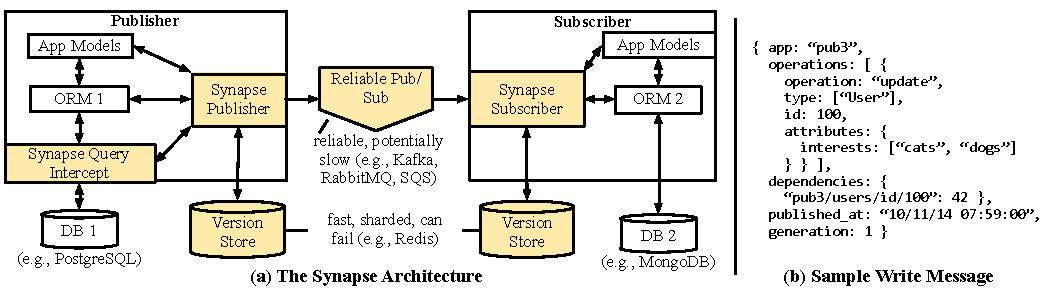
\includegraphics[width=.9\linewidth]{figures/synapse/architecture-less-detail.pdf} \vspace{-12pt}
 \caption{\small {{\bf The \synapse Architecture.}
   (a) \synapse components are shaded.  To replicate data between
       heterogeneous DBs, \synapse marshals the publisher's objects and
       sends them to subscribers, which unmarshal and save them into their
       DBs.  (b) Published message format (JSON).}}
 \label{synapse:fig:architecture}
 \vspace{-15pt}
\end{figure*}

\begin{figure}[t]
\begin{tabular}{c}
\begin{minipage}{.19\textwidth}
\vspace{-7pt}
\begin{lstlisting}[xleftmargin=1pt,framexleftmargin=1pt]
# Publisher 3 (Pub3).
# Runs on MongoDB.
class User
 include Mongoid::Document
 `\specialKeyword{publish}` do
  field :interests
 end
end
\end{lstlisting}
\end{minipage}\vspace{-8pt}\\
\begin{minipage}{.19\textwidth}
\begin{lstlisting}[xleftmargin=1pt,framexleftmargin=1pt]
# Subscriber 3a (Sub3a).
# Runs on any SQL DB.
# Searching for users based on
# interest is not supported.
class User<ActiveRecord::Base
 `\specialKeyword{subscribe}`, :from => :Pub3 do
  field :interests
 end
 serialize :interests
end
\end{lstlisting}
\end{minipage}\vspace{-8pt}\hfill
\end{tabular}
\begin{tabular}{c}
\begin{minipage}{.24\textwidth}
\begin{lstlisting}[xleftmargin=1pt,framexleftmargin=1pt]
# Subscriber 3b (Sub3b).
# Runs on any SQL DB.
# Supports searching for users by interest.
class User < ActiveRecord::Base
 has_many :interests
 `\specialKeyword{subscribe}` :from => :Pub3 do
  field :interests, :as => :interests_virt
 end
 def interests_virt=(tags)
  Interest.add_or_remove(self, tags)
 end
end
class Interest < ActiveRecord::Base
 belongs_to :user
 field :tag
 def self.add_or_remove(user, tags)
   # create/remove interests from DB.
 end
end
\end{lstlisting}
\end{minipage}
\end{tabular}
\vspace{-6pt}
\caption{{\bf Example 3: MongoDB/SQL.}
Shows one publisher running on MongoDB (Pub3) and two SQL subscribers
(Sub3a,b).  Default translations work, but may be suboptimal due to
mismatches between DBs.  Optimizing translation is easy with \synapse.
}
\label{synapse:fig:mongo-sql}
\vspace{-6pt}
\end{figure}

\heading{Example 3: Matching Data Types with Virtual Attributes.}
At times, DBs mismatch on data types.  As an example, we showcase a specific
case of integration between MongoDB and SQL.
MongoDB, a document-oriented database, has become popular among startups
lately thanks to its schemaless data model that allows for frequent
structural changes.  Since the DB imposes so little structure, importing data
into or exporting data from MongoDB is typically similar to
\label{synapse:fig:mongo-to-star}. We choose here a more corner case example to
show \synapse's applicability to complex situations.

\F~\ref{synapse:fig:mongo-sql} shows a MongoDB publisher (Pub3), which leverages a
special MongoDB feature that is not generally available in SQL,
Array types, to store user interests.  \F\ref{synapse:fig:mongo-sql} shows two options
for integrating the interests into a SQL subscriber.  The first option (Sub3a),
which works on all SQL DBs, is to serialize the array field.
In this case, we automatically flatten the array and store it in as text, which would not support efficient queries on interests.

The most straightforward solution to translate this array type to a generic SQL DB is to create an additional model, {\code \footnotesize Interest}, and a one-to-many relationship to it from {\code \footnotesize User}.
Sub3b shows how \synapse's virtual attribute abstraction easily accomplishes
this task, creating the {\code \footnotesize Interest} model and a virtual
attribute  ({\code \footnotesize interests\_virt}) to insert the new interests
received into the separate table.


\subsection{Application State Record-Replay}
\label{synapse:s:record-replay}

\synapse is an application state record-replay system and share many
similarities with application execution record-replay systems.
Under \synapse architecture (\F~\ref{synapse:fig:architecture}(a)), the
publisher application {\em records} operations that
change its state, which is entirely contained in its DB.  At a later
point in time, the subscriber {\em replays} these recorded operations mutating
its state. Considering a publisher app that publishes all of its models, and a
subscriber app running the same code as the publisher app that subscribes to all
models, the subscriber is a perfect replica of the publisher. This replica
can be used for fault-tolerance purposes, a typical use case of record-replay systems.

\synapse shares many similarities with the execution record-replay system \scribe.
Due to its go live feature, \scribe must maintain a consistent and valid OS
kernel state at any point in time during replay because the application
execution may continue uncontrolled at any point in time.
From this perspective, \scribe (resp. \synapse) records and replays the state of
the OS (resp. DB).
Table~\ref{synapse:tab:similarities} summarizes the similarities between the
two record-replay systems. The important takeaway is that both systems use a
causal engine to execute state mutation operations.

\begin{table}[t]
 \centering {\footnotesize
  \begin{tabular}{l l l}\toprule
                                     & {\bf \scribe}       & {\bf \synapse}                  \\ \midrule
Replicated state                     & OS state            & DB state                        \\
Actors                               & Userspace processes & Web app processes (distributed) \\
State mutation API                   & System calls        & DB operations                   \\
State mutation library               & libc                & DB driver                       \\
Parallelism                          & Multi-Core          & Distributed                     \\
Synchronization engine               & Causal              & Causal                          \\
Synchronization protocol             & CREW                & CREW                            \\
Synchronization primitives           & Rendezvous points   & Dependency tracking             \\
Recorded events                      & API calls           & DB data                         \\
Log format                           & Binary              & JSON                            \\
  \bottomrule
  \end{tabular}
 }
 \caption{{\small {\bf Similarities between \scribe and \synapse }}
 Each row depicts the equivalent entity with \scribe and \synapse.}
 \label{synapse:tab:similarities}
\end{table}


\section{\synapse Architecture}
\label{synapse:sec:arch}

\F~\ref{synapse:fig:architecture}(a) shows the \synapse architecture applied to an
application with a single publisher and subscriber. The publisher and subscriber
may be backed by different DBs with distinct engines, data models, or disk
layouts. In our example, the publisher runs on PostgreSQL, a relational DB,
while the subscriber runs on MongoDB, a document DB. At a high level, \synapse
marshals the publisher's model instances (i.e. objects) and publishes them to
subscribers, which unmarshal the objects and persists them through the
subscriber's ORM.

\synapse consists of two DB- and ORM-agnostic modules ({\em \synapse
Publisher} and {\em \synapse Subscriber}), which encapsulate most of the
publishing and subscribing logic, and one DB-specific module ({\em \synapse
Query Intercept}), which intercepts queries and relates them to the objects they
access. On the publisher side, \synapse interposes between the ORMs and the DB
driver to intercept updates of all published models, such as creations, updates,
or deletions of instances -- collectively called {\em writes} -- before they are
committed to the DB. The interposition layer identifies exactly which objects
are being written and passes them onto the {\em \synapse Publisher},
\synapse's DB-independent core. The Publisher then marshals all published
attributes of any created or updated objects, attaches the IDs of any deleted
objects, and constructs a {\em write message}. \synapse sends the message to a
reliable, persistent, and scalable message broker system, which distributes the
message to the subscribers. All writes within a single transaction are combined
into a single message.

The message broker reliably disseminates the write message across subscribers.
Of the many existing message brokers~\cite{jms,kafka,pubsubhubbub,rabbitmq},
we use RabbitMQ~\cite{rabbitmq} in our implementation, using it to provide a
dedicated queue for each subscriber app. Messages in the queue are processed in
parallel by multiple subscriber workers per application, which can be threads,
processes, or machines.

When a new message is available in the message broker, a \synapse subscriber
worker picks it up and unmarshals all received objects by invoking relevant
constructors and attribute setters (using the language's reflection interface).
The worker then persists the update to the underlying DB. When writing to
models, prescribed callbacks are invoked by the ORM. When transactions are
supported, the message is processed within a transaction.

\subsection{Model-Driven Replication}
\label{synapse:sec:arch:cross-db-propagation}

To synchronize distinct DBs, \synapse needs to (1) identify the objects being
written on the publisher, (2) marshal them for shipping to the subscribers, (3)
unmarshal back to objects on the subscriber side, (4) and persist them.
Although steps 1 and 4 are DB specific, we leverage ORMs to abstract the DB
specific logic.

To intercept writes, \synapse contains a DB-engine specific query interceptor.
Collecting information about objects written is
generally straightforward, as many DBs can easily output the rows affected
by each query. For example, in SQL, an {\code INSERT}, or {\code DELETE}
query ending with {\code RETURNING *} will return the contents of the
written rows. Many DBs support this feature, including: Oracle, PostgreSQL, SQL
Server, MongoDB, TokuMX, and RethinkDB. For DBs without this feature
(e.g., MySQL, Cassandra), we develop a protocol that involves performing an additional
query to identify data being written; it is safe but somewhat more expensive.

After intercepting a write, \synapse uses the ORM to map from the raw data
written back to application objects (e.g. an instance of the {\tt User} model).
The published attributes of these written object(s) are marshaled to JSON, and published
along with object dependencies (described in
\S\ref{synapse:sec:arch:cross-db-causality}) and a generation number (for recovery,
described in \S\ref{synapse:sec:arch:bootstrapping}). When marshaling objects,
\synapse also includes each object's complete inheritance tree, allowing
subscribers to consume polymorphic models.
\F~\ref{synapse:fig:architecture}(b) shows a write message produced
upon a {\code Post} creation; the post object's marshalling is in the message's
{\code attributes} field.

On the subscriber, \synapse unmarshals a new or updated object by (1)
instantiating a new instance of that type, or finding it in the DB based on its primary key with
the ORM's {\tt find} method, (2) recursively assigning its
subscribed attributes from those included in the message by calling the
object setter methods, and (3) calling the {\code save} or {\code
destroy} method on the object. For a delete operation, step (2) is skipped.
Different ORMs may have different names for these methods (e.g. {\tt find} vs
{\tt find\_by}) but their translation is trivial. Any callbacks specified by the
programmer are automatically called by the ORM.

\subsection{Enforcing Delivery Semantics} \label{synapse:sec:arch:cross-db-causality}

\synapse enforces update-message ordering with three different
delivery modes: global, causal, and weak. The performance of each delivery mode
varies, as \S\ref{synapse:sec:evaluation:delivery} will show.

\headingi{Global Ordering:}
The global ordering has the strongest delivery semantics: all publisher writes are serialized via a global lock and delivered to subscribers in order.

\headingi{Causal Ordering:}
Causal ordering identifies, for each write $W$, the prior writes that must
be applied before $W$ to avoid negative effects, such as sending a notification
for a new post to an out-of-date friends set.
\synapse implements causality in a manner very similar to other
causal systems~\cite{ahamad1995causal,Birman:1991:LCA:128738.128742,eiger,bolton}
and its dependency tracking mechanism is described in \S\ref{synapse:sec:arch:deps}.
When a publisher writes in its DB, \synapse updates causal dependency versions in its
version store and then sends the new write to the subscribers, which buffer it.
Each subscriber applies this buffered write to its DB once it has applied all
of the write's dependencies and updates its version store.
In practice, message loss may happen (see \S\ref{synapse:sec:eval:ease-of-use}), which
results in unavailable subscribers.

\headingi{Weak Ordering:}
To maintain availability despite message loss, we provide a weak
ordering mode that never blocks and offers this guarantee: as writes and
updates arrive for a document, they are always increasing.
Since \synapse transmits all published attributes (as opposed to deltas), the subscriber can always fast forward to the latest received version.

\subsection{Tracking Causal Dependencies} \label{synapse:sec:arch:deps}

To enforce causal ordering, \synapse tracks dependencies between updates.  To
first order, \synapse takes an explicit approach to identifying
dependencies, an approach that was adopted by other prior
systems~\cite{bolton,cops,Bailis:2012:PDC:2391229.2391251}.
Specifically, using two constructs in
our API, {\code with\_write\_dep} and {\code with\_read\_dep}, a developer
can specify write and read dependencies, respectively.  Each call takes as a
parameter a URI describing the dependency target. E.g.,
{\code"social\_app/ users/name/"+my\_name\_var} would reference a dependency in
the app {\code SocialApp}, on all instances of the model {\code User} that have
a {\code name} attribute equal to the app's variable, {\code my\_name\_var}.

Unlike prior work using explicit dependencies, \synapse additionally embeds
mechanisms to automatically identify dependencies.  They work well in
practice, but they may not be complete.  \synapse tracks dependencies
within the scope of individual controllers by intercepting read and write
queries and declaring a dependency from any write on all previously read objects
in the cope of that controller execution.  Similarly, all write queries
become dependent on all write queries previously executed in the scope of the
same executing controller. Between controller executions, \synapse tracks
dependencies within the scope of the user session, by including the current user
object as a dependency on all writes.  Finally, \synapse tracks dependencies
within background jobs, e.g., with Sidekiq~\cite{sidekiq}.

In many cases, \synapse can easily determine exactly which objects are read
or written by each query. \synapse automatically intercepts queries of the
form { \code SELECT x,y FROM z WHERE $<$flat expression$>$} with {\code x$=$id}
or when {\em flat expression} specifies a primary key equality constraint.
In our experience, these constitute the vast majority of true dependency
queries.  \synapse detects during testing when a read query does not match its
simple parsing structure and signals these queries to developers, who can
manually provide dependency tracking as necessary.  In the over a dozen
applications we have integrated with \synapse, we have not encountered one
single query that could be considered as a dependency but is not marked as such
by \synapse automatically.  In contrast, prior work relying on explicit
dependencies requires their use with {\em all writes}, which would believe is
onerous for developers and error-prone.

\subsection{Bootstrapping and Reliability} \label{synapse:sec:arch:bootstrapping}

When a new subscriber comes online, it must synchronize with the publisher in a
three-step bootstrapping process. First, all current publisher versions are sent
in bulk and saved in the subscriber's version store. Second, all the subscribed model
objects are sent and persisted in the subscriber's DB. Third, all the messages
published during the previous steps are processed to finish synchronizing the
objects and versions. Once all the messages are processed, the subscriber is now
{\em in sync} and operates with the configured delivery semantics.
Subscriber code may call {\code Synapse.bootstrap?} to determine whether \synapse
is still bootstrapping or in sync. \F~\ref{synapse:fig:welcome-email} shows an example of
how the mailer subscriber checks for bootstrapping completion before sending emails.

The subscriber can fail and its queue may grow to an arbitrary size. To
alleviate this issue, \synapse decommissions the subscriber from the
\synapse ecosystem and kills its queue once the queue size reaches a
configurable limit. If the subscriber comes back, \synapse initiates a
{\em partial bootstrap} to get the application back in sync.

Failures may also happen when the version store dies on either the publisher or subscriber
side. When the subscriber's version store dies, a partial bootstrap is initiated. When
the publisher's version store dies, a generation number reliably stored is incremented
and publishing resumes. Messages embed this generation number as shown on
\F~\ref{synapse:fig:architecture}(b). When subscribers see this new generation number
 in messages, they wait until all the previous generation messages are
processed. This generation change incurs a global synchronization barrier and
temporarily slows subscribers.

\subsection{Testing Framework}
\label{synapse:sec:testing}

\synapse provides a solid testing framework to help with development and
maintenance of apps.  For instance, \synapse statically checks that subscribers
don't attempt to subscribe to models and attributes that are unpublished,
providing warnings immediately. \synapse also simplifies integration testing by
reusing model factories from publishers on subscribers.  If a publisher
contains a model factory (e.g. data samples), then \synapse will seamlessly
generate integration tests by using these factories to emulate the payloads that
would be received in the subscriber app in a production environment.  This way,
developers are confident that the integration of their ecosystem of applications
is well tested before deploying into the production environment.

\setlength{\tabcolsep}{3pt}
\begin{table}[t]
 \centering {\footnotesize
  \begin{tabular}{l l l l r r}\toprule
   {\bf DB}       & {\bf ORM}    & {\bf Pub?} & {\bf Sub?} & {\bf ORM LoC} &
{\bf DB LoC} \\ \midrule
    PostgreSQL    & ActiveRecord & Y          & Y          & 474           & 44
         \\
    MySQL         & ActiveRecord & Y          & Y          & ''            & 52
         \\
    Oracle        & ActiveRecord & Y          & Y          & ''            & 47
         \\
    MongoDB       & Mongoid      & Y          & Y          & 399           & 0
         \\
    TokuMX        & Mongoid      & Y          & Y          & ''            & 0
         \\
    Cassandra      & Cequel       & Y         & Y          & 219           & 0
         \\
    Elasticsearch & Stretcher    & N/A        & Y          & 0             & 0
         \\
    Neo4j         & Neo4j        & N          & Y          & 0             & 0
         \\
    RethinkDB     & NoBrainer    & N          & Y          & 0             & 0
         \\
    Ephemerals    & N/A           & Y         & N/A          & N/A           & N/A
	\\
    Observers    & N/A           & N/A        & Y          & N/A           & N/A
         \\
  \bottomrule
  \end{tabular}
 }
 \vspace{-0.3cm}
 \caption{{\small {\bf Support for Various DBs.}
 Shows ORM- and DB-specific lines of code (LoC) to support varied DBs.
 For ORMs supporting many DBs (e.g., ActiveRecord), adding a new DB comes for free.}}
 \label{synapse:tab:db-heterogeneity}
\end{table}
\setlength{\tabcolsep}{5pt}

\subsection{Supporting New DBs and ORMs}
Adding subscriber support for a new ORM is trivial: a developer need only map the CRUD operations (create/read/update/delete) into \synapse's engine.
To add publisher support for a new ORM, a developer needs to first plug into the ORM's interfaces to intercept queries on their way to the DB (all queries for causality and writes for replication).
Then, the developer needs to add two phase commit hooks to the DB driver for transactional DBs (as discussed in \S\ref{synapse:sec:arch:bootstrapping}).

To illustrate the effort of supporting new DBs and ORMs, we report our development experience on the nine DBs listed in Table~\ref{synapse:tab:db-heterogeneity}.
Our first supported DB was PostgreSQL, taking a single developer approximately one week, and resulting in 474 lines of code specific to ActiveRecord (the ORM; for query intercept) and 44 lines specific to PostgreSQL (for two phase commit). 
After building support for this DB, supporting other SQL DBs, such as MySQL and Oracle, was trivial: about 50 lines of DB-specific, implemented in about a couple of hours for each.
Supporting subsequent DBs (e.g., MongoDB, TokuMX, and Cassandra) was equally simple and took just a few days and 200-300 lines of code per ORM.
Thus, in our experience, supporting various DBs is a very reasonable task for an experienced programmer.
\section{Applications}
\label{synapse:sec:apps}

We and others have built or modified 14 web applications to share data with
one another through \synapse.  Those built by others have been
deployed in production by a startup, \crowdtap.  The applications we built
extend popular open-source apps to integrate them into data-driven ecosystems. 
Overall, our development and deployment experience has been positive: we made
{\em no logical changes} to application code, only adding on
average a single line of configuration per attribute of each model published.
At the same time, we achieved great benefits from using \synapse.  

\subsection{\synapse at \crowdtap}
\label{synapse:sec:apps:crowdtap}

\crowdtap is an online marketing-services company contracted by major brands such as Verizon, AT\&T, Sony and MasterCard.
\crowdtap has grown rapidly since its founding, and by October 2014 has seen over 450,000 users.
As \crowdtap grew and gained more clients, both their application offering and development team evolved.

At first, engineers attempted to enhance their core application by building new features directly into the same codebase and DB.
However, as new features were added, the data was used in different ways, requiring different indexes and denormalization, bloating the DB.
When features were canceled, traces of their schema changes were often left orphaned.
Moreover, it was difficult to bring newly hired engineers up to speed with the complex and rapidly developing codebase and DB.
To alleviate this issue, engineers factored out some features and provided them
data access via synchronous APIs, but found that this technique was difficult to
get right.
Specifically, a bug in an e-commerce service, which accessed user data from
\crowdtap's core app via a synchronous API, was able to bring down the entire app due to
the lack of performance isolation.  Installing rate limits between the components
of their app was not good option for \crowdtap, and they preferred the
de-coupling that a replication-based solution cross-service would provide.
Synchronization of these DBs then became a challenge.

To address these challenges, \crowdtap began to experiment with \synapse,
first to provide synchronization between their original core app and a separate
targeting service.  These services had previously communicated over a
synchronous API; this API was factored out, and replaced with \synapse,
reducing the app from 1500 LoC to 500 LoC.  While previous attempts to integrate
this feature required the deep knowledge of the core application held by senior
engineers, this integration was performed by a newly-hired engineer.

After this initial integration, two other \crowdtap engineers extracted two other business features, the mailer and the analytics engine from the main application, instead using \synapse to provide data replication.
The email service notifies users of new actions and subscribes to 24 of the core service's models to isolate all notification related aspects within their application, while the analytics engine subscribes to a similarly complex number of models.

\crowdtap's engineering management was so pleased with the ease of development, ease of maintenance, and performance of \synapse, that after this experience, all major features have been built with it (totaling nine apps now).
\F~\ref{synapse:fig:crowdtap-ecosystem} shows the high-level architecture of the \synapse ecosystem at \crowdtap.
\synapse-related code is trivial in size and logic.
The \crowdtap main application consists of approximately 17,000 lines of ruby code, and publishes 257 attributes of 53 different models.
However, the \synapse-related configuration lines are minimal: only 360 (less
than 7 lines of configuration per model, on average).

\crowdtap has chosen different delivery semantics for their various subscribers
(shown with different arrows in \F\ref{synapse:fig:crowdtap-ecosystem}). While all
publishers are configured to support causal delivery mode, subscribers are
configured with either causal or weak delivery modes, depending on their
semantics requirements. The mailer service registers for data from
the Main app in causal mode so as to avoid sending inconsistent emails.
In contrast, the analytics engine lacks stringent order
requirements, hence it selects  a weak consistency model.

\begin{figure}[t]
\centering
   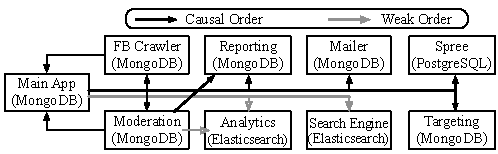
\includegraphics[width=3.3in]{figures/synapse/eco-crowdtap.pdf}
      \vspace{-20pt}
   \caption{\textbf{\crowdtap's services.} Arrows show \synapse connections.}
   \label{synapse:fig:crowdtap-ecosystem}
\end{figure}

\iffalse
\begin{figure}
\begin{minipage}{.225\textwidth}
\begin{lstlisting}[xleftmargin=3pt]
#Semantic Analyzer App (Postgres).
class User < ActiveRecord::Base
 include Synapse::Subscriber
 subscribe :email, from: 'diaspora'
 include Synapse::Publisher
 publish :interests
end
class Post < ActiveRecord::Base
 include Synapse::Subscriber
 subscribe :author_id, :public,
      :contents, from: 'diaspora'
 before_create do  #do the analysis
  #concepts attr defined in schema.
  self.concepts = Textalytics.
           analyze(contents)
 end
 after_create do  #update author
  author.interests += self.concepts
  author.save()
 end
end
\end{lstlisting}
\end{minipage}\hfill
\begin{minipage}{.225\textwidth}
\begin{lstlisting}
#Modified Spree App (MySQL).
class User < ActiveRecord::Base
 include Synapse::Subscriber
 #Subscribe to both the original
 #model and its decoration.
 subscribe :email, from: 'diaspora'
 subscribe :interests,
       from: 'diaspora_topic'
end
# Search controller.
class TargetedSearch<Spree::Search
 def get_base_scope
  tags = current_user.interests
  base_scope = super
  if tags.present?
   base_scope.reorder!('tags.count')
  end
  return base_scope
 end
end
`\ `
\end{lstlisting}
\end{minipage}
\vspace{-0.5cm}
\caption{\small {\bf Targeted Product Search for Spree.}
On the left, the Semantic Analyzer service subscribes to Diaspora and decorates
the {\code User} model with the topics of his latest posts. On the right, a
modified Spree registers for the semantic analyzer's interests decoration, and
returns products related to interests.
}
\label{synapse:fig:spree-code}
\end{figure}
\fi
\begin{figure*}[t]
 \centering \subfigure[{\bf Execution Sample:}
 \ding{172} a user posts on Diaspora. The mailer \ding{173} and semantic
 analyzer \ding{174} receive the post in parallel. Diaspora \ding{175} and Spree
 \ding{176} each receive the decorated model with in parallel.
]{ 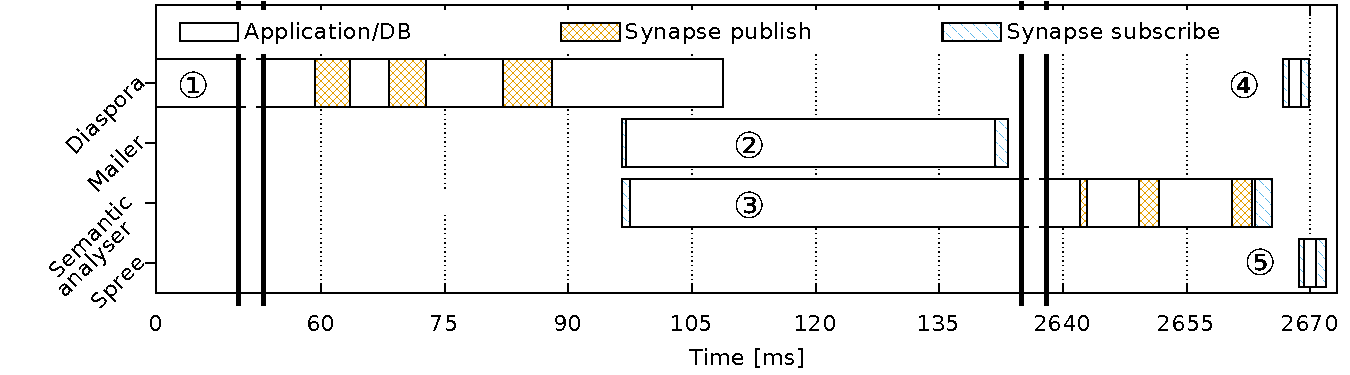
\includegraphics[width=0.48\linewidth]{figures/synapse/diaspora1.pdf}
  \label{synapse:fig:diaspora1}
 } \hfill \subfigure[{\bf Execution with Subscriber Disconnection:}
 \ding{172} and \ding{174} User 1 posts. \ding{173} and \ding{175} User 2 posts.
 Mailer comes online and processes the each users first request \ding{176}, then
 each user's second request \ding{177} in parallel.]{
   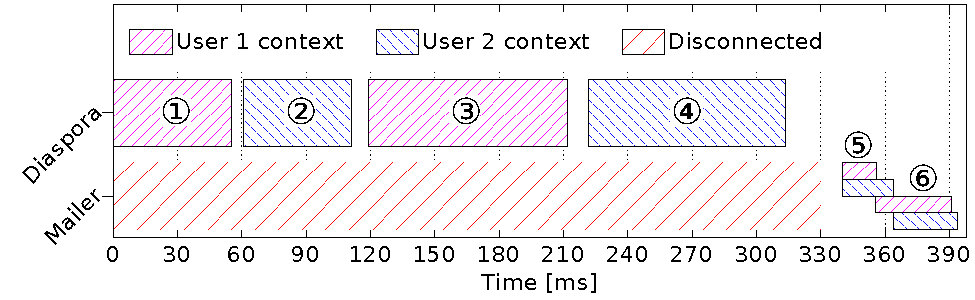
\includegraphics[width=0.48\linewidth]{figures/synapse/diaspora2.pdf}
  \label{synapse:fig:diaspora2}
 }
\vspace{-0.3cm}
 \caption{\small {\bf Execution Samples in Social Ecosystem.}
  Time grows from left to right on x axis.
  (a) Execution in the open-source ecosystem when a user posts a new message.
  (b) Execution when two users post messages with the mailer disconnected.
     }
     \vspace{-0.5cm}
\end{figure*}

\subsection{\synapse in Open-Source Apps}
\label{synapse:sec:apps:social}
\begingroup
\setlength{\columnsep}{6pt}
We used \synapse to build a new feature for \emph{Spree}, a popular open source
e-commerce application that powers over
\begin{wrapfigure}{r}{1.4in}
\centering
   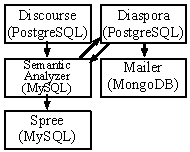
\includegraphics[width=1.2in]{figures/synapse/eco-social.pdf}
      \vspace{-6pt}
   \caption{\textbf{Social Product Recommender.} Arrows show \synapse
connections.}
   \label{synapse:fig:social-ecosystem}
\end{wrapfigure}
45,000 e-commerce websites world
wide~\cite{spree-site}.
By integrating \emph{Diaspora}, a Facebook-like open source social networking
application and \emph{Discourse}, an open source discussion board, with Spree,
we
were able to create a social-based product recommender.
\F\ref{synapse:fig:social-ecosystem} shows the architecture of the ecosystem.
We started by configuring Diaspora and Discourse to publish the models
for posts, friends, and access control lists.
We needed to add only several lines of declarative configuration each app: 23
for Diaspora (compared to its 30K lines of code), 5 for Discourse (compared to
its 21K lines), and 7 for Spree (compared to its 37K lines).

Next, we built a semantic analyzer that subscribes to these posts and extracts topics of interest, decorating Users with apparent topics of interest (using an out-of-the-box semantic analyzer, Textalytics~\cite{textalytics}).
The analyzer publishes its decorated {\code User} model (with user interests) to Spree.
\endgroup

Finally, since Spree did not have \emph{any} recommendation mechanism in place, we added several lines of code to it to implement generic targeted searching.
With this code in place, one can construct as complex a recommendation engine as
one can muster, although our prototype uses a very simple keyword-based matching
between the users' interests and product descriptions. Such code need not be
concerned with where the user's interests come from as they
automatically exist as part of the data model (thanks to \synapse).

\label{synapse:sec:examples}

\synapse addresses many of the challenges of heterogeneous-DB applications automatically through its use of ORMs, often being entirely plug-and-play.
In other cases, the programmer may need to perform explicit translations on the subscriber to align the data models.
Our experience suggests that \synapse's abstractions facilitate these translations, and we illustrate our experience using examples showcasing \synapse's usability with each major class of DB: SQL, document, analytic, and graph.

\begin{figure}[t]
\begin{tabular}{c}
\begin{minipage}{.22\textwidth}
\begin{lstlisting}[xleftmargin=1pt,framexleftmargin=1pt]
# Publisher 1 (Pub1).
# Runs on MongoDB.
class User
 include Mongoid::Document
 `\specialKeyword{publish}` do
  field :name
 end
end
\end{lstlisting}
\end{minipage}\vspace{-8pt}\\
\begin{minipage}{.22\textwidth}
\begin{lstlisting}[xleftmargin=1pt,framexleftmargin=1pt]
# Subscriber 1a (Sub1a).
# Runs on any SQL DB.
class User<ActiveRecord::Base
 `\specialKeyword{subscribe}` :from => :Pub1 do
  field :name
 end
end
\end{lstlisting}
\end{minipage}
\end{tabular}\hfill
\begin{tabular}{c}
\begin{minipage}{0.22\textwidth}
\begin{lstlisting}[xleftmargin=1pt,framexleftmargin=1pt]
# Subscriber 1b (Sub1b).
# Runs on Elasticsearch.
class User < Stretcher::Model
 `\specialKeyword{subscribe}` :from => :Pub1 do
  property :name,:analyzer=>:simple
 end
end
\end{lstlisting}
\end{minipage}\vspace{-8pt}\\
\begin{minipage}{0.22\textwidth}
\begin{lstlisting}[xleftmargin=1pt,framexleftmargin=1pt]
# Subscriber 1c (Sub1c).
# Runs on MongoDB.
class User
 include Mongoid::Document
 `\specialKeyword{subscribe}` :from => :Pub1 do
  field :name
 end
end
\end{lstlisting}
\end{minipage}
\end{tabular}
\vspace{-16pt}
\caption{{\bf Example 1: Basic Integration.}
Shows publishing/subscribing examples with actual ORMs.
\synapse code is trivial.  This is the common case in practice.
}
\label{synapse:fig:mongo-to-star}
\end{figure}

\heading{Example 1: Basic Integrations.}  Our experience suggests that most
integrations with \synapse are entirely automatic and require only simple
annotations of what should be published or subscribed, similar to the ones shown
in \F\ref{synapse:fig:pub-sub}.  To showcase, \F\ref{synapse:fig:mongo-to-star} shows the
integration of a MongoDB publisher (Pub1) with three
subscribers: SQL (Sub1a), Elasticsearch (Sub1b), and
MongoDB (Sub1c). The programmers write their models using
the specific syntax that the underlying ORM
provides.  Barring the {\code {\footnotesize publish/subscribe}} keywords, the
models are exactly how each programmer would model them if they were not using
\synapse (i.e., the data were local to their service).  In our experience
building and deploying \synapse, this is by far the most
frequent case of integration.

That said, there are at times more complex situations, where programmers must
intervene to address mismatches between schemas, supported data types, or
optimal layouts.  We find that even in these cases, \synapse provides just the
right abstractions to help the programmer address them easily and elegantly.
We describe next complex examples, which illustrate \synapse's flexibility
and great added value.  We stress that not all integrations between a given DB
pair will face such difficulties, and vice versa, the same difficulty might be
faced between other pairs than those we illustrate.

\begin{figure}
\begin{tabular}{c}
\begin{minipage}{.23\textwidth}
\begin{lstlisting}[xleftmargin=3pt]
# Publisher 2 (Pub2).
# Runs on any SQL DB.
class User<ActiveRecord::Base
 `\specialKeyword{publish}` do
  field :name
  field :likes
 end
 has_many :friendships
end
class Friendship<ActiveRecord::Base
 `\specialKeyword{publish}` do
  belongs_to :user1, :class => User
  belongs_to :user2, :class => User
 end
end
\end{lstlisting}
\end{minipage}\\
\begin{minipage}{.21\textwidth}
\vspace{0.2cm}
\caption{{\bf Example 2: SQL/Neo4j.}
Pub2 (SQL) stores friendships in their own table; Sub2 (Neo4j) stores
them as edges between Users. }
\vspace{-0.2cm}
\label{synapse:fig:sql-to-neo4j}
\end{minipage}
\end{tabular}\hfill
\begin{tabular}{c}
\begin{minipage}{.21\textwidth}
\begin{lstlisting}
# Subscriber 2 (Sub2).
# Runs on Neo4j.
class User  # persisted model
  include Neo4j::ActiveNode
  `\specialKeyword{subscribe}` :from => :Pub2 do
   property :name
   property :likes
  end
  has_many :both, :friends,
   :class => User
end
class Friendship  # not persisted
 include `\specialKeyword{Synapse::Observer}`
 `\specialKeyword{subscribe}` :from => :Pub2 do
  belongs_to :user1, :class => User
  belongs_to :user2, :class => User
 end
 after_create do
  user1.friends << user2
 end
 after_destroy do
  user1.friends.delete(user2)
 end
end
\end{lstlisting}
\end{minipage}
\end{tabular}
\end{figure}

\heading{Example 2: Mapping Data Models with Observers.}
Different DBs model data in different ways so as to optimize different modes of
accessing it. This example shows how to map the data models between a SQL and
Neo4j DB to best leverage the DBs' functions.  Neo4j, a graph-oriented DB, is
optimized for graph-structured data and queries. It stores relationships between
data items -- such as users in a social network or products in an e-commerce app
-- as edges in a graph and is optimized for queries that must traverse the graph
such as those of recommendation engines. In contrast, SQL stores relationships
in separate tables. When integrating these two DBs, model mismatches may occur.
\F\ref{synapse:fig:sql-to-neo4j} illustrates this use case with an example.

Pub2, the main application, stores Users and their friends in a SQL DB.
Sub2, an add-on recommendation engine, integrates the user and friendship
information into Neo4j to provide users with recommendations of what their
friends or network of friends liked. Its common type of query thus involves
traversing the user's social graph, perhaps several levels deep.  As in the
previous examples, we see here that the programmer defines his subscriber's User
model in the way that he would normally do so for that DB (the top of
Sub2).  However, in this case, \synapse's default translation (achieved by just
annotating data with publish/subscribe) would yield low performance since it
would store both the user and the friendship models as nodes, just like the
publisher's SQL schema does, ignoring the benefits of Neo4j.

To instead store friendships as edges in a graph between users, the programmer
leverages our observer abstraction.  She defines an observer model to
subscribe to the Friendship model, which rather than persisting the data as-is,
simply adds or removes edges among User nodes.  This solution, which involves
minimal and conceptually simple programmer input, lets the subscriber
leverage Neo4j's full power.

\begin{figure*}[t+]
 \centering 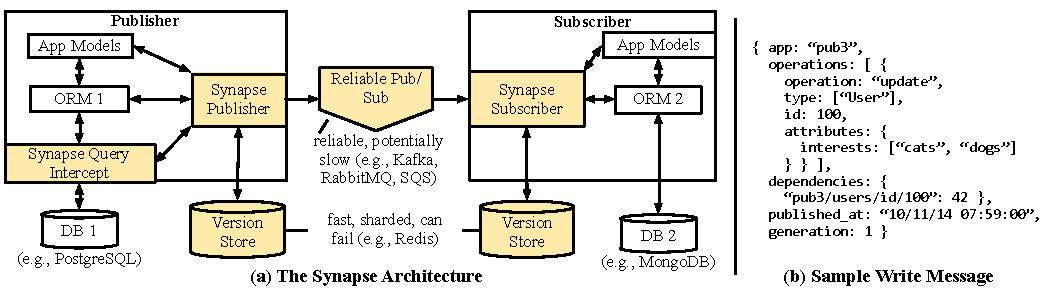
\includegraphics[width=.9\linewidth]{figures/synapse/architecture-less-detail.pdf} \vspace{-12pt}
 \caption{\small {{\bf The \synapse Architecture.}
   (a) \synapse components are shaded.  To replicate data between
       heterogeneous DBs, \synapse marshals the publisher's objects and
       sends them to subscribers, which unmarshal and save them into their
       DBs.  (b) Published message format (JSON).}}
 \label{synapse:fig:architecture}
 \vspace{-15pt}
\end{figure*}

\begin{figure}[t]
\begin{tabular}{c}
\begin{minipage}{.19\textwidth}
\vspace{-7pt}
\begin{lstlisting}[xleftmargin=1pt,framexleftmargin=1pt]
# Publisher 3 (Pub3).
# Runs on MongoDB.
class User
 include Mongoid::Document
 `\specialKeyword{publish}` do
  field :interests
 end
end
\end{lstlisting}
\end{minipage}\vspace{-8pt}\\
\begin{minipage}{.19\textwidth}
\begin{lstlisting}[xleftmargin=1pt,framexleftmargin=1pt]
# Subscriber 3a (Sub3a).
# Runs on any SQL DB.
# Searching for users based on
# interest is not supported.
class User<ActiveRecord::Base
 `\specialKeyword{subscribe}`, :from => :Pub3 do
  field :interests
 end
 serialize :interests
end
\end{lstlisting}
\end{minipage}\vspace{-8pt}\hfill
\end{tabular}
\begin{tabular}{c}
\begin{minipage}{.24\textwidth}
\begin{lstlisting}[xleftmargin=1pt,framexleftmargin=1pt]
# Subscriber 3b (Sub3b).
# Runs on any SQL DB.
# Supports searching for users by interest.
class User < ActiveRecord::Base
 has_many :interests
 `\specialKeyword{subscribe}` :from => :Pub3 do
  field :interests, :as => :interests_virt
 end
 def interests_virt=(tags)
  Interest.add_or_remove(self, tags)
 end
end
class Interest < ActiveRecord::Base
 belongs_to :user
 field :tag
 def self.add_or_remove(user, tags)
   # create/remove interests from DB.
 end
end
\end{lstlisting}
\end{minipage}
\end{tabular}
\vspace{-6pt}
\caption{{\bf Example 3: MongoDB/SQL.}
Shows one publisher running on MongoDB (Pub3) and two SQL subscribers
(Sub3a,b).  Default translations work, but may be suboptimal due to
mismatches between DBs.  Optimizing translation is easy with \synapse.
}
\label{synapse:fig:mongo-sql}
\vspace{-6pt}
\end{figure}

\heading{Example 3: Matching Data Types with Virtual Attributes.}
At times, DBs mismatch on data types.  As an example, we showcase a specific
case of integration between MongoDB and SQL.
MongoDB, a document-oriented database, has become popular among startups
lately thanks to its schemaless data model that allows for frequent
structural changes.  Since the DB imposes so little structure, importing data
into or exporting data from MongoDB is typically similar to
\label{synapse:fig:mongo-to-star}. We choose here a more corner case example to
show \synapse's applicability to complex situations.

\F~\ref{synapse:fig:mongo-sql} shows a MongoDB publisher (Pub3), which leverages a
special MongoDB feature that is not generally available in SQL,
Array types, to store user interests.  \F\ref{synapse:fig:mongo-sql} shows two options
for integrating the interests into a SQL subscriber.  The first option (Sub3a),
which works on all SQL DBs, is to serialize the array field.
In this case, we automatically flatten the array and store it in as text, which would not support efficient queries on interests.  ORMs, such as

The most straightforward solution to translate this array type to a generic SQL DB is to create an additional model, {\code \footnotesize Interest}, and a one-to-many relationship to it from {\code \footnotesize User}.
Sub3b shows how \synapse's virtual attribute abstraction easily accomplishes
this task, creating the {\code \footnotesize Interest} model and a virtual
attribute  ({\code \footnotesize interests\_virt}) to insert the new interests
received into the separate table.

\subsection{Splitting a monolithic app into services with \synapse}
\label{synapse:sec:apps:gitlab}

We used \synapse to split an open source monolithic application, GitLab, into a
service oriented architecture application. GitLab is a source revision system
frontend similar to GitHub.  GitLab is built on Ruby-on-Rails and used by more
than 100,000 companies.  With \synapse, we were able to extract all email
functionality into a separate service, independent of the core application,
running on its own database.

We extracted 276 lines from GitLab core application into the mailer.  10 models
had to be published out of a total of 22.  To increase our confidence that the
extraction was successful, we leveraged \synapse testing framework. We were able
to migrate 124 tests cases (700 lines of code) related to the mailer from the
GitLab core application to the extracted mailer service.  We did not have to
rewrite or modify any of these test cases.  \synapse transparently reuse the
data factories to mock \synapse messages as if they were received from the main
application, exactly like it would happen in a deployed system. These passing
test cases demonstrate the correctness of the feature extraction into its own
service.

However, the mailer sometimes needs to render the output of a {\tt git diff} on
a specific repository. Because git repositories are not replicated, the mailer
must communicate with the main application through a synchronous API to
retrieve computation on git repositories.

\section{Evaluation}
\label{synapse:sec:evaluation}

We leverage both our deployment and the applications we built to answer three
core evaluation questions about \synapse: (Q1) How expensive is it
on the publisher side? (Q2) How well does it scale? (Q3) How do its various
delivery modes compare? and (Q4) How useful is it in practice?

To answer these questions, we ran experiments on Amazon AWS with up to 1,000
c3.large instances (2-core, 4GB) running simultaneously to saturate \synapse.
As workloads, we used a mix of \crowdtap production traffic and microbenchmarks
that stress the system in ways that production workload cannot.  Unless
otherwise noted, our evaluation focuses on the causal delivery mode, which is
the default setting in our prototype.  After providing some sample executions,
we next discuss each evaluation question in turn.

\subsection{Sample Executions}
\label{synapse:sec:evaluation:sample-runs}

To build intuition into how \synapse behaves and the kinds of overheads it
brings, we show two sample executions of our open-source ecosystem
applications (see \S\ref{synapse:sec:apps:social}). All applications are configured
with a causal delivery mode, hence the examples reflect this mode's functioning.

Figure~\ref{synapse:fig:diaspora1} shows a timeline of the applications' execution
starting with a user's post to Diaspora and ending with Spree's receipt of the
semantically-enhanced User model. We observe that \synapse delivers messages
shortly after publication (within 5ms), in parallel to both the mailer and
the semantic analyzer.  Figure~\ref{synapse:fig:diaspora2}  illustrates visually
\synapse's causal engine in action. It shows two users posting messages on
different Diaspora profiles app while a Mailer subscriber is deployed to notify
a user's friends whenever the user makes a new post.  Initially, the mailer is
disconnected. When the mailer comes back online, it processes messages from the
two users in parallel, but processes each user's posts in serial order, thereby
enforcing causality.

\setlength{\tabcolsep}{4pt}

\subsection{Application Overheads (Q1)}
\label{synapse:sec:evaluation:overhead}

We next evaluate \synapse's publishing overheads in the context of real
applications: \crowdtap and the open-source apps we modified. For \crowdtap, we
instrumented \crowdtap's main Web application to record performance metrics and
recorded accesses to the application over the 24 hour period of April 16th,
2014. In total, we recorded one fifth of the traffic totaling 170,000 accesses
to application controllers. For each controller, we measured the average
number of published messages, the average number of dependencies per message
published, the average execution time of the controller, and the average
\synapse overhead, compared to the raw controller latency. This workload is
realistic, however it is not high enough to bottleneck \synapse. We evaluate
the scalability of \synapse directly in \S\ref{synapse:sec:evaluation:scalability}.

\begin{figure*}[t]
 \subfigure[c][{\bf \synapse Overheads at \crowdtap}]{ \raisebox{2.1cm}
{\footnotesize
     \begin{tabular}{l|r|r|r|r|r} \hline
    {\bf Most Popular} & {\bf \% Calls}  & {\bf Published}                     &
\multicolumn{1}{c|}{{\bf Avg.}} & {\bf Controller} & \multicolumn{1}{c}{{\bf
\synapse}}    \\
     {\bf Controllers} & {\bf (of 170k)} & \multicolumn{1}{c|}{{\bf Messages}} &
{\bf \# Deps}                   & {\bf Time (ms)}  & \multicolumn{1}{c}{{\bf
Overhead (ms)}} \\ \hline

      awards/index  & 17.0\% & 0.00 & 0.00  & 56.5  & 0.01 (0.03\%)  \\
     brands/show    & 16.0\% & 0.03 & 0.06  & 97.0  & 0.61 (0.60\%)  \\
     actions/index  & 15.0\% & 0.67 & 13.31 & 170.0 & 12.00 (7.00\%) \\
     me/show        & 12.0\% & 0.00 & 0.00  & 14.7  & 0.00 (0.00\%)  \\
     actions/update & 11.5\% & 3.46 & 9.79  & 240.0 & 65.00 (27.0\%) \\

       \hline
     \multicolumn{6}{l}{ {\bf Average overhead across all 55 controllers:}
4.40\%, standard deviation=8.80\% }
       \vspace{-45pt}
      \end{tabular}
     }
     \label{synapse:tab:crowdtap-overheads}
    }
    \hspace{1cm}
    \subfigure[c][{\bf \synapse Overheads in Real Applications}]{
     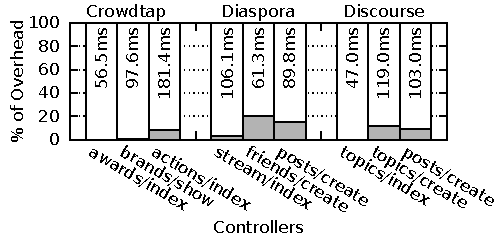
\includegraphics[width=7cm]{figures/synapse/overhead-hist.pdf}
     \label{synapse:fig:app-overheads}
    }
\vspace{-10pt}
    \caption{\small {\bf Application Publishing Overheads.}
      (a) \crowdtap dependencies and overheads, sampled from production data.
          For each of the five most frequently invoked controllers in \crowdtap,
          shows the percent of calls to it, average number of published
          messages, average number of dependencies between messages,
          the average controller execution time, and the average overhead from
          \synapse.
      (b) \synapse overhead (gray parts) for 3 controllers in 3 different
          applications. Labels give the total controller times.
          {\em \synapse publisher overheads are small.}
    }
    \vspace{-15pt}
   \end{figure*}
\setlength{\tabcolsep}{5pt}

   \begin{figure*}[t]
    \centering \subfigure[{\bf Publisher Overhead vs. Dependencies}]{
      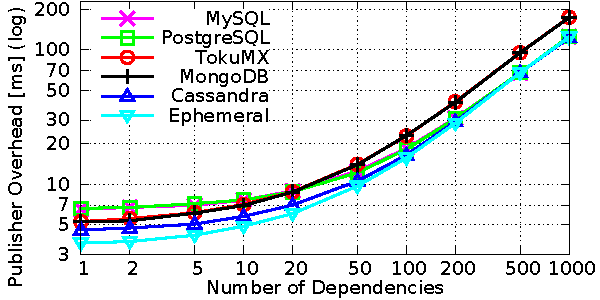
\includegraphics[width=0.31\linewidth]{figures/synapse/overheadvsdeps.pdf}
      \label{synapse:fig:overhead}
    } \hspace{0.1cm} \subfigure[{\bf Throughput on Different DBs}]{
      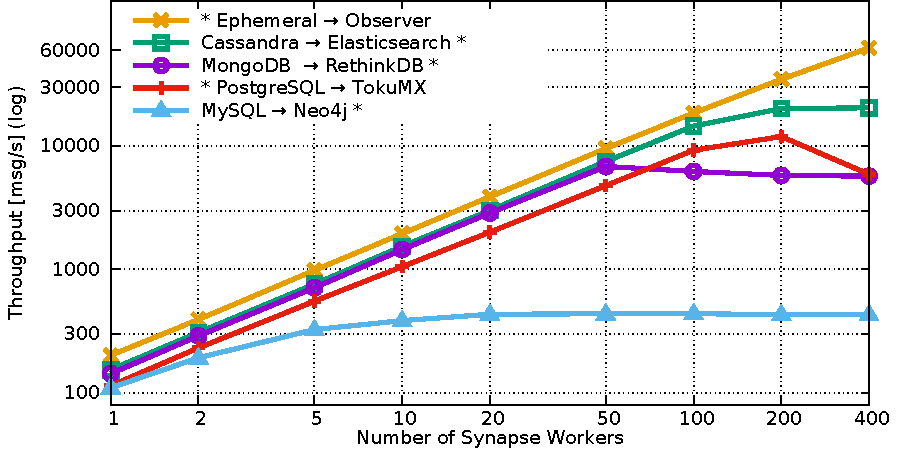
\includegraphics[width=0.31\linewidth]{figures/synapse/db-throughput-vs-workers.pdf}
      \label{synapse:fig:dbs-throughput}
    } \hspace{0.1cm} \subfigure[{\bf Throughput on Various Delivery Semantics}]{
      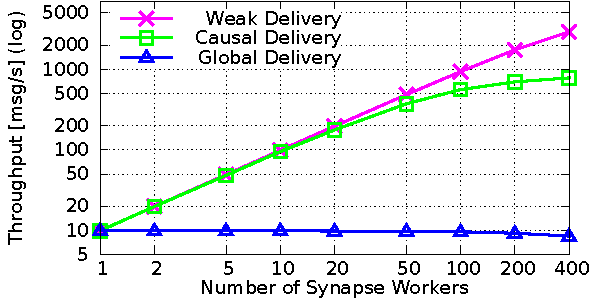
\includegraphics[width=0.31\linewidth]{figures/synapse/throughputvsworkerssaturate.pdf}
      \label{synapse:fig:parallel-throughput}
    }
    \vspace{-0.4cm}
    \caption{\small {\bf Microbenchmark Results.}
     (a) Publisher overhead on different DBs.
     (b) Throughput vs number of workers end to end benchmark.
         Each line represents a different DB setup.
         The slowest end in each pair is annotated with a (*) symbol.
     (c) Throughput vs number of workers with subscribers running a 100ms callback.
         Each line represents a different delivery mode.
         {\em Causal and weak delivery modes scale well.}
     \vspace{-15pt} }
   \end{figure*}

Figure \ref{synapse:tab:crowdtap-overheads} shows our results. In total, 55 controllers
were invoked. We show average overheads across them, as well as detailed
information about the five most frequently accessed controllers, which account
for over 70\% of the traffic. On average, \synapse overheads are low: 4.4\%.
For the most popular two controllers ({\code awards/index} and {\code
brands/show}), the overheads are even lower: 0.03-0.6\%. This is because they
exhibit very few published messages (writes). As expected, \synapse overhead
is higher in controllers that publish more messages, showing a maximum overhead
of 27\% for the controller {\code actions/update}. The number of dependencies also
impacts the overhead, with the controller {\code actions/index} showing a 7\%
overhead for 13.31 dependencies on average per update in that controller.

To complement our \crowdtap results, we measured controllers in our opens-source
applications, as well. Figure \ref{synapse:fig:app-overheads} shows the \synapse
overheads in for several controllers within Diaspora and Discourse (plus
\crowdtap for consistency). Grey areas are \synapse overheads. Overheads
remain low for the two open-source applications. Read-only controllers, such as
{\code stream/index} and {\code topics/index} in Diaspora and Discourse,
respectively, exhibit near-zero overheads; write controllers have up to 20\%
overhead.

These results show that \synapse overheads with real applications are low and
likely unnoticeable to users. However, the results are insufficient to assess
performance under stress, a topic that we discuss next.

\subsection{Scalability (Q2)}
\label{synapse:sec:evaluation:scalability}

To evaluate \synapse throughput and latency under high load, we developed a
stress-test microbenchmark, which simulates a social networking site. Users
continuously create posts and comments; comments are related to posts and create
cross-user dependencies. We issue traffic as fast as possible to saturate \synapse, with a
uniform distribution of 25\% posts and 75\% comments. We run this experiment
by deploying identical numbers of publishers and subscribers (up to 400 for
each) in Amazon AWS. As persistence layers, we use several of our supported
DBs and combinations. We applied different DBs as publishers and
subscribers. We measure a variety of metrics, including the overheads for
creating a post, as well as \synapse's throughput.

\heading{Overheads under Heavy Load.}
\F~\ref{synapse:fig:overhead} shows the overheads for different DBs with increasing
numbers of dependencies. Focusing on the one-dependency case (x=1), \synapse
adds overheads ranging from 4.5ms overhead on Cassandra to 6.5ms on PostgreSQL.
This is in comparison to the 0.81ms and 1.9ms latencies that PostgreSQL and
Cassandra, respectively, exhibit {\em without} \synapse. However, compared to
realistic Web controller latencies of tens of ms, these overheads are barely
user-visible. As the number of dependencies increases, the overhead grows slowly
at first, remaining below 10ms for up to 20 dependencies. It then shoots up to a
high 173ms for 1,000 dependencies. Fortunately, as shown in
Figure~\ref{synapse:tab:crowdtap-overheads}, dependencies in real applications remain
fairly low (below 13 on average for \crowdtap).

\heading{Cross-DB Throughputs.}
\F~\ref{synapse:fig:dbs-throughput} shows how \synapse's end-to-end throughput scales
with the number of publisher/subscriber workers, for various DB
combinations, as well as for our
DB-less models (observer to ephemeral). We keep the number of dependencies per
message constant at 4 and shard the version stores on 80 AWS instances. We have not sharded
any of the DBs. For ephemerals, \synapse scales linearly with the number of
workers, reaching a throughput of more than 60,000 msg/s. Even at such high
rates, \synapse does not become a bottleneck.  When DBs are used to
back the publishers and subscribers, the throughput grows linearly with the
number of workers until one of the DBs saturates. Saturation happens when the
slowest of the publisher and subscriber DBs reaches its maximum throughput. The
figure marks with a * the DB that bottlenecks in each combination. For
instance, PostgreSQL bottlenecks at 12,000 writes/s, and Elasticsearch at
20,000 writes/s.

\subsection{Delivery Semantic Comparison (Q3)}
\label{synapse:sec:evaluation:delivery}

\synapse supports three delivery modes -- global, causal, and weak -- which
provide different scaling properties.
\F\ref{synapse:fig:parallel-throughput} compares subscriber scalability with 
increased number of subscriber workers available to process writes in parallel.
We configure subscribers with a 100-ms callback delay to simulate
denormalization and DB commits.  The global delivery mode, which requires the
subscriber to commit each write serially, scales poorly.  The causal
delivery mode, which only requires the subscriber to serialize dependent
updates, provides much better scalability.  Its peak throughput is limited by
the inherent parallelism of the workload.  Finally, the weak delivery mode
scales perfectly, never reaching its peak up to 400 subscriber workers.
In practice, we recommend choosing either the causal or weak mode.

\subsection{Production Notes (Q4)}
\label{synapse:sec:eval:ease-of-use}

As stated before, \crowdtap has given us very positive feedback on \synapse's
usability and value.  We next relate several interesting stories from
their use of \synapse in production:

\headingi{Supports Live Migrations:} \crowdtap discovered a new use for
\synapse that we had not anticipated.  They used it to implement live DB
migrations.  Unhappy with MongoDB's performance, they migrated their Main App to
TokuMX, another document-oriented DB.  To do so, they bootstrapped a subscriber
app implementing the same functionality as the original app but running on
TokuMX. The subscriber registered for all the Main App's data.  Once it was up
to date, developers just switched their load balancer to the new application and
the migration was completed with little downtime.  They also applied this
mechanism to address otherwise difficult schema migration challenges.

\headingi{Supports Agile Development:} A key aspect in a startup company is
agility.  New features must be rolled out quickly and securely evaluated.
According to \crowdtap, \synapse helps with that. One developer said: ``It
allows us to be very agile. We can experiment with new features, with real
data coming from production.''  For example, during a hackathon, one of the
developers implemented a new reporting prototype. He was able to subscribe to
real time production data without impacting the rest of the system thanks to
\synapse's isolation properties. The business team immediately adopted this
reporting tool, and has been using it ever since.

\headingi{Flexible Semantic Matters:} Interestingly, \crowdtap initially
configured all of its services to run in causal mode.  However, during an
upgrade of RabbitMQ, the (otherwise reliable) message queuing system that
\synapse relies upon, some updates were lost due to an upgrade failure.
Two subscribers deadlocked, and their queues were filling up, since they were
missing dependencies and could not consume the updates.  After timeouts, \synapse's
recovery mechanisms, which rebootstrap the subscribers, kicked in
and the system was unblocked.  However, the subscriber apps were unavailable for
a long period of time. \crowdtap now chooses between causal and weak delivery
modes for each of its subscribers, taking into account its availability/consistency
needs.  It is not an easy choice, but according to them, it {\em can} and {\em must}
be done in a production environment where even reliable components can fail.

\subsection{Summary}

We have shown that \synapse is easy to integrate with applications,
and can support multiple, different DBs with reasonable effort. \synapse adds
reasonable overhead on real applications, and is not a bottleneck for
scalability.  Moreover, although still a research prototype, it has been shown
to be valuable beyond its initial promise in production.

\section{Related Work}
\label{synapse:sec:related}

\synapse builds upon an immense body of work spanning multiple fields,
including systems, DBs, and software engineering. The major relevant
directions of prior research are: DB replication, data warehousing, federated
DBs, pub/sub systems, and consistency models. We adopt various techniques from
these areas, but instantiate them in unique ways for the domain of modern
MVC-based applications. This lets us break through challenges incurred by more
general prior approaches, and design the first real-time service integration
system that supports both SQL and NoSQL DBs with simple APIs, strong semantics,
and good scalability.

\heading{Same-DB Replication.}
The vast majority of work in DB replication (a good survey of which can be found
in Cecchet, et.al.~\cite{candea-db-replication}) involves replicating data
across different instances of {\em the same DB engine} to increase the DB's
availability, reliability, or throughput.  Traditional DB replication systems
plug in at low levels~\cite{candea-db-replication}, which makes them DB
specific: e.g., they intercept updates inside their engines (e.g., Postgres
replication~\cite{postgres-r}), between the DB driver and the DB engine (e.g.,
MySQL replication~\cite{mysql-replication}), or at the driver level (e.g.,
Middle-R~\cite{middle-r}).  \synapse operates at a much higher level -- the
ORM -- keeping it largely independent of the DB.

\heading{Data Warehousing and Change Capture Systems.}
Data warehousing is a traditional approach for replicating data across
heterogeneous DBs~\cite{books/daglib/0029346,Chaudhuri:1997:ODW:248603.248616}.
While many warehousing techniques~\cite{Chan:1999:DSM:319757.319787,10.1109/TKDE.2005.16,Yang:1997:AMV:645923.673657,dynamo-es-river,mongo-es-river,mosql} are not suitable for
real-time integration, change-data capture systems, one class of data
warehousing systems, are focused on real-time transfer of data updates
between different DB engines. 
Moreover, most traditional data warehousing systems, developed by the DB
community, are focused on replicating data between different SQL DB vendors.
Replication is usually implemented either by installing
triggers that update data in other DBs upon local updates, or by tailing the
transaction log and replaying it on other DBs, as LinkedIn's Databus
does~\cite{databus}.

Triggers are unfortunately not supported by NoSQL DBs, which invalidates this approach for our purposes.
For instance, although the SymmetricDS \cite{symmetricDS} project supports synchronizing data \emph{to} a MongoDB subscriber, it can not replicate data \emph{from} a MongoDB publisher.
Although transaction logs are often supported, it is
generally agreed that parsing these logs is extremely fragile and difficult,
since the logs are proprietary and not guaranteed to be stable across version
updates~\cite{databus}.  \synapse differs from all of these systems by
replicating at the level of ORMs, a much more generic and stable layer, which
lets it replicate data between both SQL and NoSQL engines.

In general, existing systems for replicating between SQL and NoSQL DBs, such as MoSQL \cite{mosql}, MongoRiver \cite{mongo-es-river} and DynamoRiver \cite{dynamo-es-river} work between only specific pairs of DBs, and offer different programming abstractions, semantics and delay properties (most in fact are non-realtime).
In contrast, \synapse provides a novel, unified framework for integrating
many DB types in realtime.

\heading{DB Federation.}
The DB community has long studied the general topic of integrating data from
different DBs into one application, a topic generally known as DB
federation~\cite{ramakrishnan2003database}. Like \synapse, federation systems
establish a translation layer between the different DBs, and typically rely on
DB views -- materialized or not -- to perform translations.  Some systems even
leverage ORMs to achieve uniform access to heterogeneous
DBs~\cite{conf/otm/BalstersH09}. However, these systems are fundamentally
different from \synapse: they let the {\em same} application access data
stored in different DBs uniformly, whereas \synapse lets {\em different}
applications (subscribers) replicate data from one DB (the publisher).  Such
replication, inspired by service-oriented architectures, promotes isolation
and lets the subscribers use the best types of DBs, indexes, and layouts that
are optimal for each case.

Similar to DB federation is projects that aim to create ``universal'' ORMs, which definite a common interface to all DBs (SQL or otherwise), such as Hibernate \cite{hibernate}, DataMapper \cite{datamapper} and CaminteJS \cite{camintejs}.
Such ORMs should in theory ease development of an application that accesses data across different DBs, a problem complementary to that which \synapse solves.
However, since they expose a purely generic interface, such an ORM will encourage a design that does not cater to the individual features provided by each DB.
In contrast, \synapse encourages developers to use different ORMs for different sorts of DBs, providing a common programming abstraction to replicate the data across them.

\heading{Publish/Subscribe Systems.}
\synapse's API is inspired by publish/subscribe systems, a long-time active
area of research~\cite{siena,scribe,thialfi,gryphon,pubsubhubbub,hermes}.
\synapse also incorporates a reliable messaging system,
RabbitMQ~\cite{rabbitmq}, but could use other systems that ensure eventual and
scalable dissemination of messages to subscribers~\cite{kafka,scribe}.
All of these systems require programmers to both specify which messages should
be included in which unit of order, while \synapse contexts {\em
transparently} intercepts data updates, compiles their dependencies
automatically, and publishes them.

\heading{Causality.}
Many consistency models have been developed, which establish varied tradeoffs
between the safety properties of the system (e.g., the accuracy and freshness of
reads) versus its availability and scale~\cite{brewer-conj}.
Among these consistency models, causal
consistency~\cite{Lamport:1978:TCO:359545.359563}
has been demonstrated to provide a good balance between semantics and
scalability~\cite{cops,eiger} and is the strongest model achievable with high
availability under network partitions~\cite{mahajan11cacTR}.  Many
implementations of causal consistency exist in the context of
{\em same-DB replication}~\cite{eiger,cops,bolton,Du:2013:OSC:2523616.2523628,Belaramani:2006:PR:1267680.1267685,Ladin:1992:PHA:138873.138877,bayou,zawirski13swiftcloud,Wang:2013:RSS:2482626.2482661,Birman:1991:LCA:128738.128742}.  \synapse applies these approaches to provide
causal order of update delivery between {\em distinct DBs}.

\section{Conclusion} \label{synapse:sec:conclusion}

\synapse is an easy-to-use, strong-semantics cross-DB system for
large-scale, data-driven web service integration. It leverages high-level
abstractions of web application frameworks, Models and Controllers. Models
provided by ORMs are used to equip \synapse of a common translation layer
compatible with many SQL and NoSQL DBs. Controllers are used to
support application-specific consistency semantics.
We have implemented \synapse for Rails
applications, demonstrated that it provides highly scalable performance,
released it open source on GitHub, and deployed it in production
to run the Web services for a company.

